\documentclass[10pt,twocolumn,letterpaper]{article}

\usepackage{cvpr}
\usepackage{times}
\usepackage{epsfig}
\usepackage{graphicx}
\usepackage{amsmath}
\usepackage{amssymb}

% Include other packages here, before hyperref.

% If you comment hyperref and then uncomment it, you should delete
% egpaper.aux before re-running latex.  (Or just hit 'q' on the first latex
% run, let it finish, and you should be clear).
\usepackage[pagebackref=true,breaklinks=true,letterpaper=true,colorlinks,bookmarks=false]{hyperref}

% \cvprfinalcopy % *** Uncomment this line for the final submission

\def\cvprPaperID{****} % *** Enter the CVPR Paper ID here
\def\httilde{\mbox{\tt\raisebox{-.5ex}{\symbol{126}}}}

% Pages are numbered in submission mode, and unnumbered in camera-ready
\ifcvprfinal\pagestyle{empty}\fi
\begin{document}

%%%%%%%%% TITLE
\title{Using fine-grain detection to understad society}

\author{First Author\\
Institution1\\
Institution1 address\\
{\tt\small firstauthor@i1.org}
% For a paper whose authors are all at the same institution,
% omit the following lines up until the closing ``}''.
% Additional authors and addresses can be added with ``\and'',
% just like the second author.
% To save space, use either the email address or home page, not both
\and
Second Author\\
Institution2\\
First line of institution2 address\\
{\tt\small secondauthor@i2.org}
}

\maketitle
%\thispagestyle{empty}

%%%%%%%%% ABSTRACT
\begin{abstract}
Detecting a large number of BMWs in images informs us that those images may be of a wealthy area. Conversely, knowing that our images were obtained from a wealthy neighborhood increases the likelihood of detecting expensive cars. We explore this relationship between demographic factors and fine-grain classes by performing large scale detection of over 2600 car classes and conducting a social analysis of unprecedented scale in computer vision. Using 45 million images from 200 of the biggest cities in the United States,we predict demographic factors such as neighborhood wealth and crime statistics. Finally we show that just as fine-grain classes provide demographic information, societal cues can assist in fine-grain classification and improve accuracy. To facilitate our work, we have collected the largest and most challenging fine-grain dataset reported to date consisting of 3147 classes of cars comprised of images from google street view and other web sources and classified by car experts to account for even the most subtle of visual differences. We hope our work ushers in a new research area fusing fine-grained object detection and societal analysis.
\end{abstract}

\section{Introduction}
%%%%%%%%% BODY TEXT
The ubiquity of street view images has jumpstarted a new line of computer vision research focused on understanding cities through images \cite{mit_plos_1}~\cite{MIT_vision}~\cite{tamara}. For example, \cite{mit_plos_1} showed that crime predictions can be improved by incorporating human perceptions of neighborhoods' images rather than using census data such as income alone~\cite{mit_plos_1} and ~\cite{tamara} and \cite{MIT_vision} learn these perceptions using computer vision techniques. However, in order to extend these methods to other cities,extensive annotations of millions of images from each city would be required since, as ~\cite{tamara} showed, algorithms trained on images of Boston, for example, cannot predict safety or wealth on images from San Francisco.  We explore the question of learning social priors using large scale fine-grain classifications of cars and show that many neighborhood statistics such as income and crime rate can be predicted from car detections. Furthermore, using our detections in conjunction with census data, we can answer questions like what types of cars do rich/poor people drive? 

\begin{figure}[t]
\begin{center}
\fbox{\rule{0pt}{2in} \rule{0.9\linewidth}{0pt}}
   %\includegraphics[width=0.8\linewidth]{egfigure.eps}
\end{center}
   \caption{some pull figure}
\label{fig:pull}
%\label{fig:onecol}
\end{figure}

Finally we show that we can use the answers to these questions to help improve fine-grained classification. Although an increasing number of images that we interact with daily are associated with GPS tags, there are very few computer vision algorithms that take advantage of location based metadata. This metadata can be especially important in fine grain classification. For example, just as detecting a large number of expensive cars in one area can give us a hint that we are in the vicinity of a wealthy neighborhood, knowing that we are in a wealthy neighborhood can also increase our likelihood of detecting expensive cars. Similarly, knowing that we are in a farm area increases our likelihood of detecting farm related cars and seeing many family households with young children increases our likelihood of detecting SUVs. We show that this information can be leveraged to improve fine-grain classification. Although there has been previous work on learning spatio-temporal priors for fine-grain classification~\cite{birdsnap} and exploiting street view geometry and GIS systems to improve object detection~\cite{nyc3D,amir} to our knowledge this is the first time census data and other social cues have been used to assist in fine-grain classification.  


Summarizing our contributions:
  \begin{enumerate}
    \item We perform a large scale analysis of cities using our car detections and present intuitive as well as interesting insights
    \item We show that using social cues extracted from census data can improve fine-grain classification accuracy
    \item We present the largest fine-grain car dataset reported to our knowledge, complete with geotags and class as well as geography metadata  
    \item We include a larger set of 45 million street view images with car detections and fine-grain class predictions
  \end{enumerate}

%------------------------------------------------------------------------
\section{Related Work}
\textbf{Analysis of cities using images.}
  \begin{enumerate}
     \item Plos one journal from MIT asking people to predict whether an area is safe/wealthy etc... after looking at the images
     \item streetscore MIT paper predicting safety wealth scores etc.. just from images~\cite{MIT_vision}
     \item tamara Berg's paper on safety on ECCV
     ~\cite{zhang2014part}
     ~\cite{caltech_birds}

\textbf{Using GPS data to improve object detection.}
     \item Amir's work in GIS assisted object detections. For objects like streetlamps and trashcans, uses GIS to reproject objects to a plane and reduce the search space for object detection .
     \item NYC 3D uses geographic elevation data to create view-point aware detectors and extract ground planes for  them
     \item Birdsnap fine-grain dataset with spatio-temporal prior for birds

  \end{enumerate}

%------------------------------------------------------------------------
\section{Cars and Cities dataset}
Our dataset consists of W number of images annotated with bounding boxes and fine-grained classes for training and validating fine-grained car detectors and 45 million street view images for societal analysis.

\subsection{Images with Labeled fine-grained classes}
Out of the images annotated with fine-grained classes and bounding boxes, X were obtained from google street view, Y from craigslist.com and Z from cars.com. A of our images have bounding boxes for cars and B are annotated with fine-grain labels. The bounding boxes were obtained through a series of AMT tasks. The fine-grain labels were created by first coming up with a class list of 18000 cars comprising of all cars listed on edmunds.com and grouping them into visually indistinguishable sets of groups using a series of amazon mechanical turk tasks as well as manual labor by the authors. After creating an exhaustive class list of 3147 classes, images from craigslist and cars.com were labeled by parsing the posting titles while cars from google street view were labeled using 100 hired car experts.

\begin{figure}[t]
\begin{center}
\fbox{\rule{0pt}{2in} \rule{0.9\linewidth}{0pt}}
   %\includegraphics[width=0.8\linewidth]{egfigure.eps}
\end{center}
   \caption{Example images from our data}
\label{fig:dataset1}

\end{figure}

\begin{figure}[t]
\begin{center}
\fbox{\rule{0pt}{2in} \rule{0.9\linewidth}{0pt}}
   %\includegraphics[width=0.8\linewidth]{egfigure.eps}
\end{center}
   \caption{Image statistics from our data}
\label{fig:dataset2}

\end{figure}

\begin{figure}[t]
\begin{center}
\fbox{\rule{0pt}{2in} \rule{0.9\linewidth}{0pt}}
\end{center}
   \caption{Some fine-grain car classes are very visually similar}
\label{fig:dataset3}
\end{figure}

Fig.~\ref{fig:dataset1} shows example images from our data while Fig.~\ref{fig:dataset2} shows some image statistics. Images from craigslist.com and cars.com have one large bounding box whereas google street view images have multiple small boxes with cars that are blurred and occluded. As shown in Fig.~\ref{fig:dataset3} the different fine-grain classes are very difficult to distinguish

\subsection{Images with no labeled fine-grained classes}
In order to perform societal analysis, we collected 45 million google street view images from 8 million points in 200 of the biggest cities in the United States. These images were collected by sampling latitude,longitude points on roads, spaced 25 meters apart. Fig.~\ref{fig:dataset4} shows maps from two cities with the samples that were collected and fig.~\ref{fig:dataset5} shows the number of samples for the 10 biggest cities. For each sample, we collect images at 0,60,120,180,240,300 degrees.

\begin{figure}[t]
\begin{center}
\fbox{\rule{0pt}{2in} \rule{0.9\linewidth}{0pt}}
   %\includegraphics[width=0.8\linewidth]{egfigure.eps}
\end{center}
   \caption{Maps of Boston and San Francisco, each dot represents a sample image in our data}
\label{fig:dataset4}
\end{figure}

\begin{figure}[t]
\begin{center}
\fbox{\rule{0pt}{2in} \rule{0.9\linewidth}{0pt}}
   %\includegraphics[width=0.8\linewidth]{egfigure.eps}
\end{center}
   \caption{The number of latitude, longitude samples for 10 cities with the most number of samples}
\label{fig:dataset5}
\end{figure}

\section{Car detection and fine-grained classification}
In order to detect and classify 45 million images, we need to use an efficient car detection and classification algorithm. Although RCNN ~\cite{rcnn} has been shown to be state of the art in object detection, it's memory and computation requirement make it impossible for use in a large scale detection problem such as ours. Specifically training with RCNN  would require XXXXGB of memory and XXXX GPUs and car detection on 45 million images would take XXminutes per bounding box on XXX machine. We therefore used a simple DPM model with 0 components to detect cars and a standard CNN from ~\cite{alexnet} to perform classification on the detected bounding boxes. As shown in Fig.~\ref{fig:dpm_acc} there is only an XX\% drop in average precision between using a dpm with 0 components and 0 parts and one with XXX components and YYY parts.

\begin{figure}[t]
\begin{center}
\fbox{\rule{0pt}{2in} \rule{0.9\linewidth}{0pt}}
   %\includegraphics[width=0.8\linewidth]{egfigure.eps}
\end{center}
   \caption{Average precision Vs. number of components and number of parts for DPM}
\label{fig:dpm_acc}
\end{figure}

In order to classify the detected cars, we train a standard CNN from ~\cite{alexnet} using caffe ~\cite{caffe}. Although our aim is to train fine-grain detections for street view images, many of our training images are obtained from other web sources due to the fact that annotating street view images is expensive. Thus we apply various deformations such as blurring in an attempt to make the web images more similar to street view images. During test time, we classify the top 10\% scoring dpm bounding boxes using our CNN. This speeds up classification time by 10X while only resulting in a drop of .5 AP. 

\section{Societal analysis}
\label{sec:social}
After collecting data, training fine-grained car detectors and classifying cars in all of our images, we now have all the components to perform social analysis. We show some general results from the entire united states as well as case studies from cities we could obtain ground truth data for. We divide our analysis into different sections below.

\subsection{What cars on the street tell us about people}

\subsubsection{Cars on the street versus cars people drive}
The first question we asked is how do cars on the street relate to the cars that people drive? Specifically,
can we learn about the registered cars in a zipcode from our street view detections?
In order to answer this question we downloaded the vehicle census from Massachusettes, which is the only state to release extensive vehicle registration data. Surprisingly, we found an extremely high pearson correlation coefficient of 0.9 (p value=XXX) between the number of cars we detected per zipcode and the number of cars that are registered per zipcode in the three cities we analysed in Masachusettes: Boston, Worcester and Springfield. The high correlation was only obtained after aggregating cars at the zip code level which tells us that most people in these cities must drive within their zip code. 
After establishing a high correlation between the number of cars we detect and the number of registred cars, we also measured the correlation between the make of the detected and registered cars per zip code. As we can see in fig.~\ref{fig:ma_corrs} there is a high correlation for most of the makes. This shows us that the cars we detect from street view images can actually tell us a lot about the types of cars that people in a particular zipcode drive.

\begin{figure} [t]
\begin{center}
\includegraphics[width=1\linewidth]{img/boston_make_corr.png}
\end{center}
\caption {Pearson correlation coefficient and p values between the number of detected and registered cars in Boston for each make.}
\label{fig:ma_corrs}
\end{figure}


\begin{figure}[t]
\begin{center}
%\fbox{\rule{0pt}{2in} \rule{0.9\linewidth}{0pt}}
   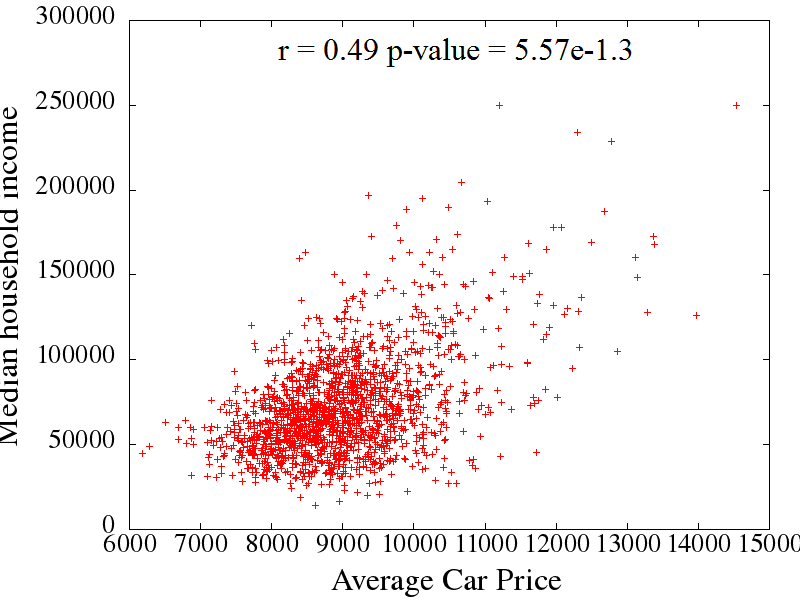
\includegraphics[width=0.8\linewidth]{img/averagePriceIncome.png}
\end{center}
   \caption {Average car price w.r.t. median household income.}
\label{fig:price-income-corr}
%\label{fig:onecol}
\end{figure}

\subsubsection{What do rich/poor people drive?}
We gathered zip code level as well as census tract level 2007-2012 American Community Survey data for the 200 cities in our dataset and analyzed how the census data relates to statistics from our detected cars. 

Table \ref{table:car-census-corrs} shows correlation values between various attributes of the detected cars and median household income per zipcode. Fig.~\ref{fig:price-income-corr} shows a plot of median household income vs. average car price in a zipcode. As expected, the highest correlation is between median household income and the average car price per zipcode (r=0.59, p \(\sim\) 0). This makes sense since rich people mostly live around places with expensive cars and tend to drive expensive cars. Our results also indicate that rich people prefer to drive foreign, especially German cars (r=0.59). This observation is also consistent with our expectations since expensive cars such as BMWs are German. What is perhaps surprising is that there is a very high negative correlation (r=-0.55, p \(\sim\) 0) between the percentage of American cars in a zip code and median household income. So poor people live in places with many American cars.

Poor people also live near very old cars where as rich people live near newer ones. As table \ref{table:car-census-corrs} shows, the correlation between median household income and the number of cars in 1990-1994 is very negative and increases to a high positive 0.59 for cars in the 2005-2009 range. Finally, a perhaps not surprising result is that poor people live near cars with low miles per gallon (MPG). This corroborates~\cite{cal-traffic-study} study showing that poor people are more exposed to car pollution than rich people.
 

\begin{table}
\begin{center}
\begin{tabular}{|l|c|}
\hline
Method & Frobnability \\
\hline\hline
Theirs & Frumpy \\
Yours & Frobbly \\
Ours & Makes one's heart Frob\\
\hline
\end{tabular}
\end{center}
\caption{Pearson correlation coefficient between various census variables and detected car attributes. All p values are \(\sim\) 0}
\label{table:car-census-corrs}
\end{table}

\subsubsection{How does education relate to cars on the street?}
One would probably guess that there is a high negative correlation between the number of people with only a high school education and the average price of a car in a zipcode. Indeed, we found that this is the case (r=0.3 p \(\sim\) 0). As expected, we also found a high correlation between the number of college educated people in a zip code and the average car price. What is perhaps surprising is that although there is a large increase in correlation coefficient as we go from high school to college educated, the jump from college to graduate school is very low (r=0.31 for college educated and 0.39 for graduate school). This tells us that there is a very low difference in the price of cars driven by people who only hold bachealors as opposed to graduate degrees.

\subsection{What cars on the street tell us about neighborhoods}
\subsubsection{Which neighborhoods are wealthy/poor?}
We ask the question: what can our street view car detections tell us about the wealth of a neighborhood? Specifically, can we predict which neighborhoods are wealthy/unwealthy using our detections? Intuitively, if we see many expensive cars on the street, we suspect that we are in a rich neighborhood and vice versa. However, the correlation between car prices and neighborhood wealth is not going to be perfect because we are not necessarily detecting the cars that are registered by residents. Figure \ref{fig:bos-sf-vis} A shows a heat map of the average price of detected cars within a zip code and median household income in a zip code for Boston and figure \ref{fig:bos-sf-vis} B shows the same visualization for San Francisco. We can see that in both cities, the average car price in a zipcode is a very good predictor of wealthy/unwealthy neighborhoods.

\subsubsection{Which neighborhoods have high car pollution?}
Can our street view detections tell us anything about which neighborhoods are affected by highly polluting cars? To answer this question, we plotted a heatmap of the expected number of cars per sample inversely weighted by the expected MPG of that sample. Using this simple measure we should be able to have a rough idea of the location of highly polluting neighborhoods. For the same density of cars, areas with high MPG result in lower numbers than those with low MPG. For different densities of cars, the relative magnitude of the measure depends on both the density of cars and how efficient they are. Fig.~\ref{fig:pollution}A shows the density of cars in San Francisco and B shows the pollution heatmap that we created. Although we could not find ground truth data of car pollution, Fig.~\ref{fig:pollution}C is a map of San Francisco air quality measuring annual average particulate matter concentration (MPG) from all sources. Our maps seems to aggree with their data in most cases.

\begin{figure*}[t]
\begin{center}
  \raisebox{-.02\height}
 {
   \includegraphics[width=0.3\linewidth]{img/sf_density.png}
 }
   \includegraphics[width=0.3\linewidth]{img/sf_mpg.png}
   \includegraphics[width=0.3\linewidth]{img/sf_air_cropped.png}
\end{center}
   \caption {A. Density of cars in San francisco, B. Our measure of car pollution in San Francisco, C. Ground Truth for Air quality (measured in annual particulate matter) in San Francisco.}
\label{fig:pollution}
\end{figure*}

\subsection{What cars on the street tell us about cities}
\subsubsection{Which cities are more segregated?}
In this section we ask the question: which cities show high clustering of similarly priced cars? Specifically, which cities have expensive cars clustered together with other expensive cars and cheap cars clustered with other cheap cars? Given the high correlation between meidan household income and average car price, the answer to this question should give us a good indication of the cities that are most and least segregated. Following the analysis of ~\cites{mit_plos_1} we use the Moran I statistic to measure spatial autocorrelation where a value of 1 indicates perfect clustering of similar values, -1 indicates perfect dispersion and 0 indicates random spatial arrangement (neither clustering nor dispersion). Fig.~\ref{fig: moran-i} plots the highest and lowest scoring cities as well as well as others in between. We can see that Houston shows the highest clustering where as Las Vegas shows the lowest

\subsubsection{Which cities are patriotic?}
Which cities have the most number of domestic cars? As Fig.~\ref{city_price} shows the coastal cities have a high concentration of foreign made cars where as the midwest has a low concentraion. This result is to be expected since the coasts also have a higher number of immigrants as well as a higher concentration of wealthy people. And as we showed in our previous analyses, wealthy people tend to drive foreign cars.

\subsubsection{Which cities are wealthy?}
In our final analysis, we ask which city has the most expensive cars on average? Fig.~\ref{city_price} maps the average car price for each city. We can see that many of the east coast cities have expensive cars as well as some cities in the south like Atlanta. We found the city with the most expensive cars to be New York and the one with the least expensive cars to be El Paso. The fact that our results predict New York may not be surprising given that some of the wealthiest people in the United States live there and those who are less wealthy tend to take public transportation.


\begin{figure}[t]
\begin{center}
    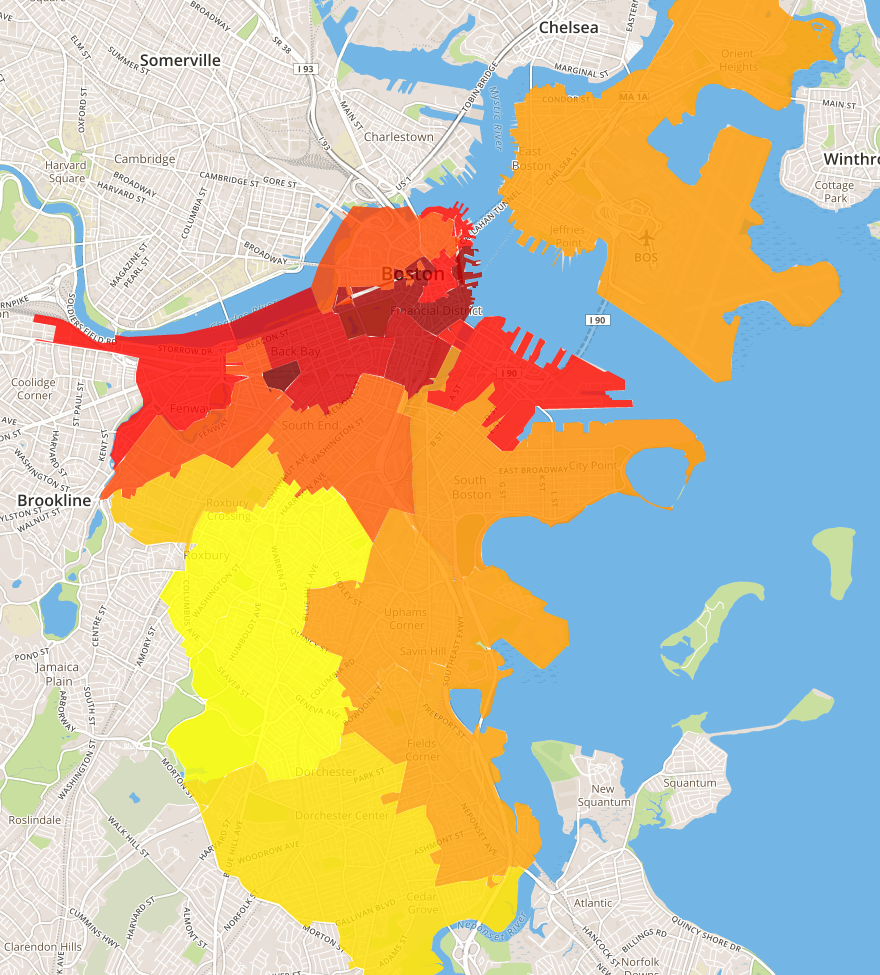
\includegraphics[width=0.45\linewidth]{img/price.png}
    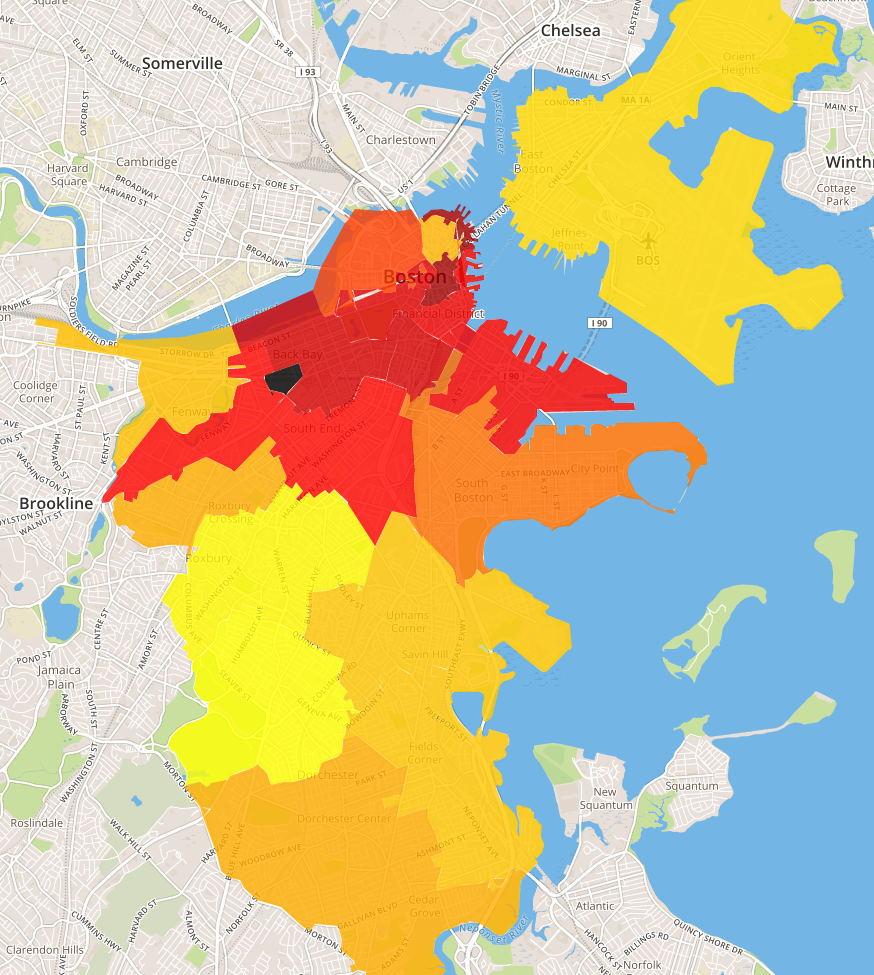
\includegraphics[width=0.45\linewidth]{img/income.png}
    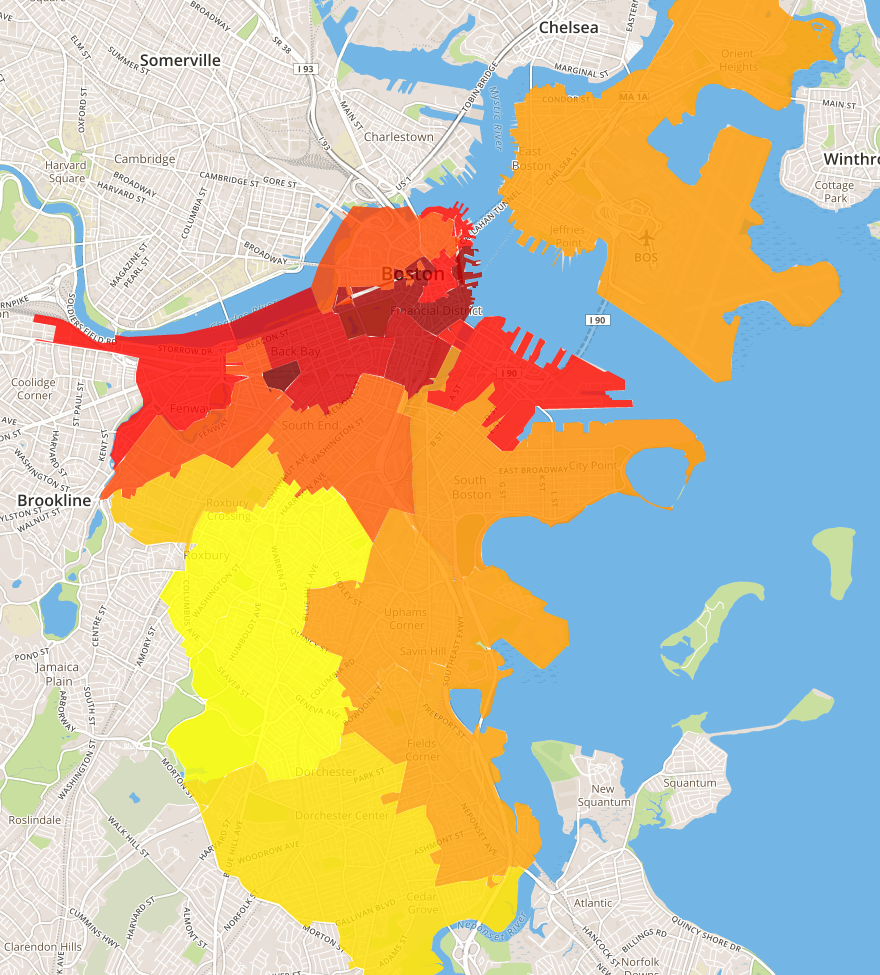
\includegraphics[width=0.45\linewidth]{img/price.png}
    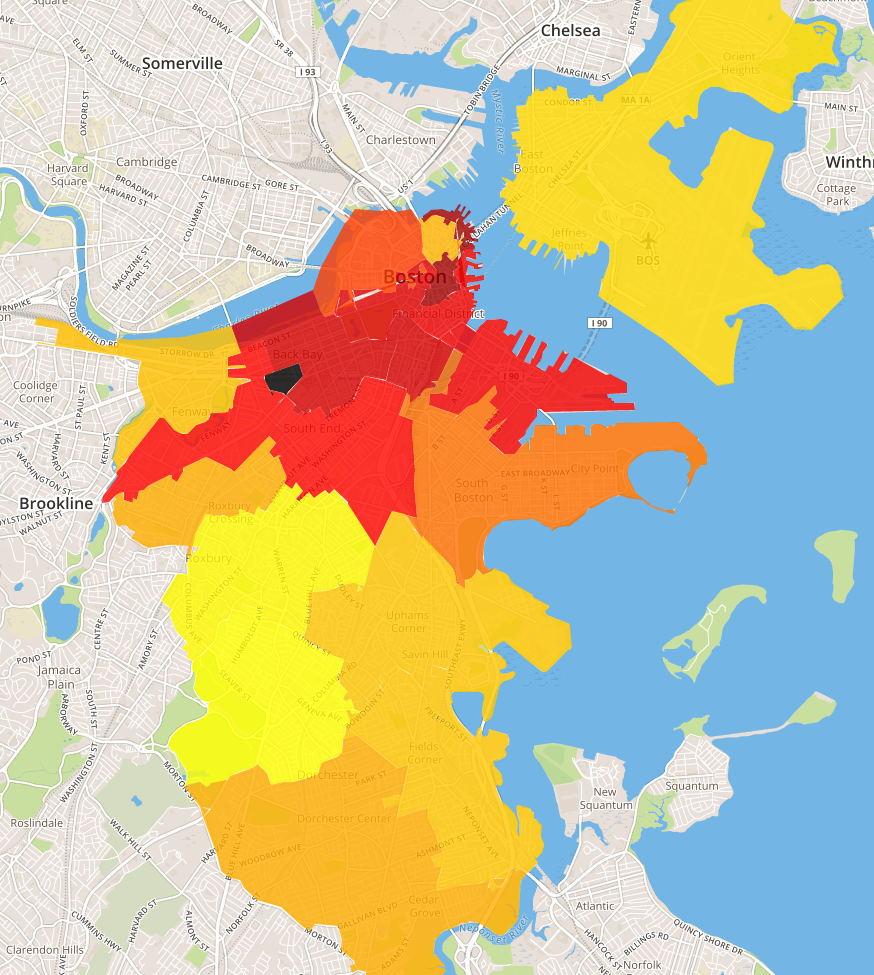
\includegraphics[width=0.45\linewidth]{img/income.png}
\end{center}
   \caption {(A) Heatmap of average car price in Boston. (B) Heatmap of median household income in Boston}
\label{fig:bos-sf-vis}
\end{figure}

\begin{figure}[t]
\begin{center}
    \includegraphics[width=0.45\linewidth]{img/city_foreign.png}
    \includegraphics[width=0.45\linewidth]{img/city_price.png}
\end{center}
   \caption {A. Map of the percentage of foreign cars in each city.San Francisco has the highest percentage and Casper the lowest. B.Map of the United States showing the expected car price in each city. New York has the highest expected car price where as El Paso has the lowest.
\label{fig:city_price}
\end{figure}

\section{Using social priors to improve classification}
As shown in section ~\ref{sec:social} there is a very high correlation between some census variables such as income, and car attributes such as price and year. Given this relationship, we explore the use of census data to improve our fine-grain classification.

\subsection{Analyzing classification accuracy}
Since census data is most highly correlated with aggregate car attributes, one question is how much knowing ground truth car attributes would help in classification accuracy. This gives us an upper bound for the gain in accuracy that can be obtained by using census variables as a prior. Table~\ref{table:car-att} lists the classification accuracy after using ground truth car attributes. Surprisingly, knowing the manufacturing country of the car gives very little gain in accuracy (\(\sim\) 0.5\%). However, localizing the car price to within one of two bins of expensive vs cheap cars provides a gain in accuracy of ~3\%. Looking at the confusion matrices in fig. ~\ref{fig:fg-confusion} we can see that after dividing the car price into 5 bins using quantiles, some expensive cars are confused with cheap cars where as most car countries of origin are not confused with other countries, except for one case of confusion between South Korean and Japanese cars.

\begin{figure*}[t]
\begin{center}
   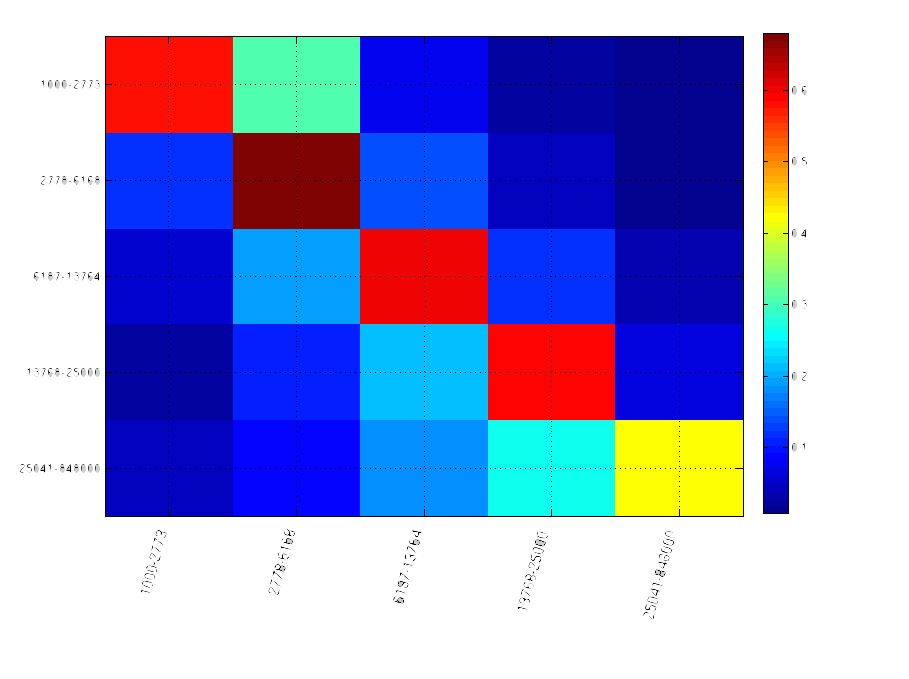
\includegraphics[width=0.4\linewidth]{img/confusion_price5.png}
   \hspace{0.1\linewidth}
   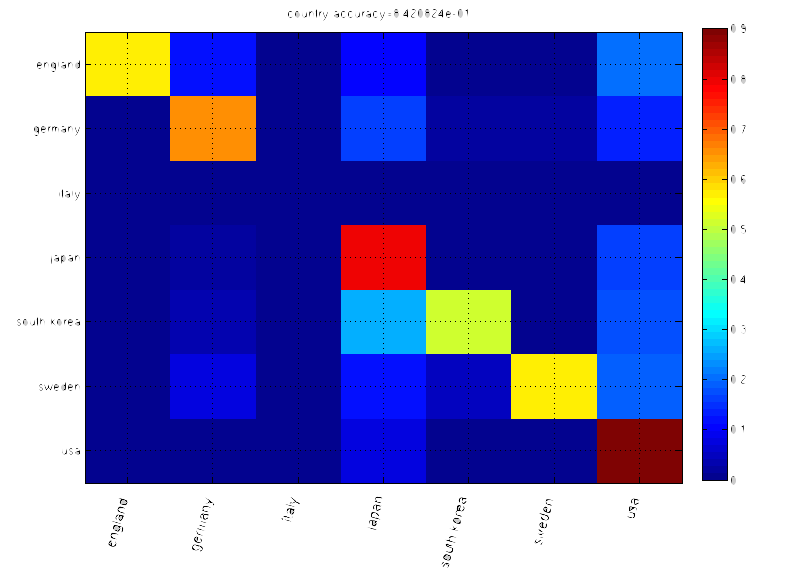
\includegraphics[width=0.4\linewidth]{img/confusion_country.png}
\end{center}
   \caption{(A) Confusion matrix between different price bins. Cheap cars are mistaken for expensive cars (B) Between cars made in different countries}
\label{fig:fg-confusion}
\end{figure*}

We take this experiment further and plot accuracy Vs. price bin in fig.~\ref{fig:price-acc} for various numbers of price bins, all generated using quantiles, localized to various degrees of accuracy. For example, we can see that if we localize
 the price of the car to one of 4 bins we would get an 8\% increase in classification accuracy. However, even localizing 
the price to within 3 out of those 4 bins would result in a ~1\% increase.


\begin{table}
\begin{center}
\begin{tabular}{|l|c|}
\hline
Method & Frobnability \\
\hline\hline
Theirs & Frumpy \\
Yours & Frobbly \\
Ours & Makes one's heart Frob\\
\hline
\end{tabular}
\end{center}
\caption{Classification accuracy with ground truth attributes}
\label{table:car-att}
\end{table}

\begin{figure}[t]
\begin{center}
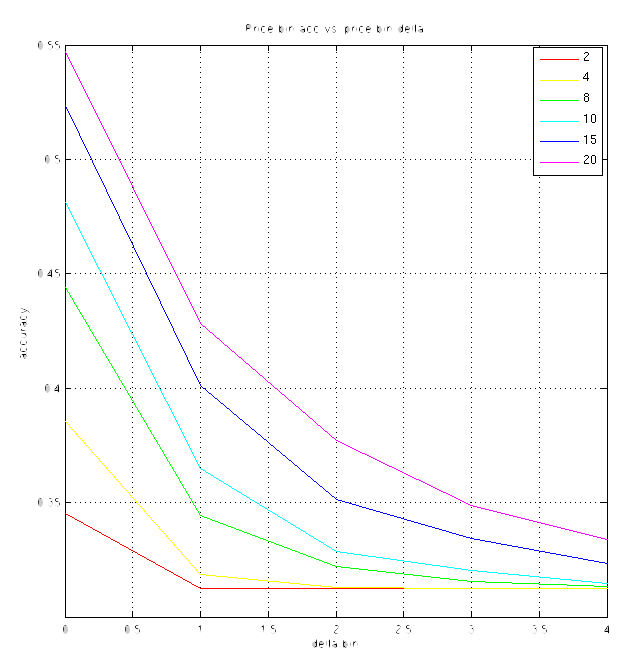
\includegraphics[width=0.9\linewidth]{img/price-att.png}
\end{center}
   \caption{Fine-grain classification accuracy with ground truth price bin. X axis is the number of bins to which the price is localized and Y axis is classification accuracy. For example, localizing the price to 3 out of 8 bins results in a classification accuracy of 33\% which is 2\% higher than the baseline, 31.27\%}
\label{fig:price-acc}
\end{figure}

\subsection{Using census priors to predict attributes}
\label{sec:prior-att}
As shown in ~\cite{birdsnap} ~\cite{Other context stuff} using contextual priors can improve object classification accuracy. In order to directly use census information as a prior, we would like to find \(P(C|I,Sk)\) where \(C\) is the fine-grain class,\(I\) is an image and \(Sk\) \(\in\) \(\{\)\(S1\) \ldots \(Sn\)\(\}\) is a particular zip code level census variable such as median household income. Using Bayes' rule:
\begin{equation}
P(C|I,Sk)=\frac{P(I,Sk|C)P(C)}{P(I,Sk)}
\end{equation}
If we assume that the image and census data are conditionally independent given the fine-grained class label, the above equation can be written as 
\begin{equation}
P(C|I,Sk)=\frac{P(I|C)P(Sk|C)P(C)}{P(I,Sk)}
\end{equation}
After applying Bayes' rule again to \(P(I|C)\) and \(P(Sk|C)\) , we get 
\begin{equation}
P(C|I,Sk)=\frac{P(C|I)P(I)}{P(C)}\frac{P(C|Sk)P(Sk)}{P(C)} \frac{P(C)}{P(I,Sk)}
\end{equation}
\begin{equation}
\propto \frac{P(C|I)}{P(C)}P(C|Sk)
\label{eq:prior-eq}
\end{equation}

We experimented with different methods of using census variables as priors. The first method was to quantize them into varying numbers of bins and calculate \(P(C|Sk)\) in equation ~\ref{eq:prior-eq} for each census variable.As shown in table ~\ref{table:prior-acc} this method results in a reduction in accuracy because we do not have enough geotagged training data to gain informative knowledge from the census about one of 2657 fine-grain classes. However, although there are 2657 classes, the number of attribute classes is much lower. If \(Aj\) \(\in\) \(\{\) \(A1\) \ldots \(An\)\(\}\) represents a car attribute such as price, we can reformulate \(P(C|Sk)\) in equation~\ref{eq:prior-eq} as \(P(C|Aj)\)\(P(Aj|Sk)\). This formulation comes from a naive bays generative model assuming that \(Sk\) are the observed variables from which we can calculate \(P(Aj|Sk)\). After this modification, equation ~\ref{eq:prior-eq} can be written as


\begin{equation}
  P(C|I,Sk) \propto \frac{P(C|I)}{P(C)}P(C|Aj)P(Aj|Sk)
\end{equation}
We calculate \(P(C|I,Sk)\) for all car attributes and 30 different census variables, quantizing them into bins ranging from 2-20. Table~\ref{table:prior-acc} shows the 3 highest accuracy numbers for various combinations of census variables and car attributes. It can be seen that using median household income and either car price or year result in the highest accuracy gain (although this gain is very slight). This result is to be expected given the social analysis results of section~\ref{sec:social} showing high correlation between median household income and car price and year.


\subsection{Multiple car attributes and census variables}
In section \ref{sec:prior-att} we used single car attributes and census variables to calculate prior probabilities. We also experimented with using multiple census variables to predict single car attributes as well as combining priors independently calculated from multiple census variables and car attributes. To obtain \(P(Aj|S1...Sn)\) we first quantize attributes \(Aj\) into \(M\) bins where \(M\) ranges from 2 to 20. If \(Aj\) has a fixed number of classes (such as car make), \(M\) is just the number of attribute classes. We then perform multi-class logistic regression along with feature selection to classify \(Aj\) into one of \(M\) bins using \(S1\) \ldots \(Sn\). \(P(Aj|S1\) \ldots \(Sn)\) is then the probability obtained through logistic regression.

Finally, we combine the priors learned for different attributes by using the fact that car attributes are independent from each other given the class. Using this assumption along with Bayes’ rule \(P(C|A1 \ldots An)\) can be written as 

\begin{equation}
\frac{P(A1\ldots An|C)P(C)}{P(A1\ldots An)}
\end{equation}
After making use of the conditional independence of \(A1\) \ldots \(An\) given \(C\) this becomes
\begin{equation}
\frac{P(C)}{P(A1\ldots An)}\prod\limits_{j=1}^n P(Aj|C)
\end{equation}
And after applying Bayes’ rule to \(P(Aj|C)\) we get 
\begin{equation}
\propto \frac{P(C)}{P(A1\ldots An)}\prod\limits_{j=1}^n P(C|Aj)
\end{equation}

We assume that car attributes are independent from each other given census variables. \(P(C|I,S1 \ldots Sn)\) is then  

\begin{equation}
\propto \frac{P(C)}{P(A1\ldots An)}\prod\limits_{j=1}^n P(C|Aj)P(Aj|S1...Sn)
\end{equation}

Where \(P(Aj|S1...Sn)\) is given by the logistic regression probabilities.

Table XXX shows the accuracies obtained after combining multiple census attributes and multiple car attributes. ***Maybe more descussion after experiments***
\begin{table}
\begin{center}
\begin{tabular}{|l|c|}
\hline
Method & Frobnability \\
\hline\hline
Theirs & Frumpy \\
Yours & Frobbly \\
Ours & Makes one's heart Frob\\
\hline
\end{tabular}
\end{center}
\caption{Results.Ours is better.}
\label{table:prior-acc}
\end{table}

\section{Conclusion}
{\small
\bibliographystyle{ieee}
\bibliography{egbib}
}

\end{document}

{\small
\bibliographystyle{ieee}
\bibliography{egbib}
}
\end{document}


